\subsection{Privacy Analysis}
\label{subsec:l2_dp}
The overall goal is to translate an $(\eps, \delta)$-DP privacy budget to the minimum $\sigma$ such that the $\ell_2$ mechanism $M$ with parameter $\sigma$ satisfies $(\eps, \delta)$-DP. To do this, we focus on a subroutine that determines whether or not $M$ satisfies $(\eps, \delta)$-DP and then binary search over $\sigma$.

Recall from \Cref{lem:approx_dp} that $M$ is $(\eps, \delta)$-DP if and only if $\P{}{\ell_{M,X,X'} \geq \eps} - e^\eps\P{}{\ell_{M,X',X}  \leq -\eps} \leq \delta$. The next subsections will provide algorithms that upper bound the first term and lower bound the second term, and thus err on the side of a conservative privacy guarantee.

Before starting our privacy analysis, we consider a simpler (but, as we will see, significantly worse) approach. The $\ell_2$ mechanism, and the $K$-norm mechanism more broadly, can be viewed as instances of the exponential mechanism~\cite{MT07}. The exponential mechanism admits a few possible approximate DP analyses. For example, the $\eps$-DP exponential mechanism satisfies $\frac{\eps^2}{8}$-concentrated DP~\cite{CR21}, and a concentrated DP guarantee can be converted to an approximate DP guarantee~\cite{BS16, CKS20, ALCKS20, ZDW22}. However, any such analysis also applies to the Laplace mechanism, and the $\eps$-DP Laplace mechanism is only $(\eps', \delta)$-DP for $\eps' \approx \eps - O(\delta)$ (\Cref{lem:laplace_approx} in the Appendix). This is a negligible improvement for realistic $\delta$, so a different privacy analysis is necessary.

\subsubsection{First Term Upper Bound}
\label{subsubsec:ub}
For the privacy guarantee to hold, \Cref{eq:iff} must hold for arbitrary neighboring databases $X$ and $X'$. Since the $\ell_2$ ball is spherically symmetric, without loss of generality we consider statistic $T$ where $T(X) = 0$ and $T(X') = e_1 = (1, 0, \ldots, 0)$. Shorthand the respective mechanisms as $M(0)$ and $M(1)$. Then
\begin{align*}
    \ell_{M,X,X'}(y) =&\ \ln\left(\frac{f_X(y)}{f_{X'}(y)}\right) \\
    =&\ \ln\left(\frac{\exp[-\|y\|_2 / \sigma]}{\exp[-\|y - e_1\|_2 / \sigma]}\right) \\
    =&\ \frac{1}{\sigma}\left(\|y-e_1\|_2 - \|y\|_2\right)
\end{align*}
so we want to upper bound
\begin{equation}
\label{eq:plrv_1_ub}
    \P{y \sim M(0)}{\frac{1}{\sigma}\left(\|y-e_1\|_2 - \|y\|_2\right) \geq \eps}.
\end{equation}
We shorthand the relevant region in \Cref{eq:plrv_1_ub} as $V$.
\begin{definition}
\label{def:V}
    Define $V = \{y \mid \frac{1}{\sigma}(\|y-e_1\|_2 - \|y\|_2) \geq \eps\}$, $M$'s \emph{high privacy loss region}.
\end{definition}
A simple case is $\sigma \geq \frac{1}{\eps}$.
\begin{lemma}
\label{lem:large_sigma}
    $\sigma \geq \frac{1}{\eps}$ if and only if $\P{y \sim M(0)}{y \in V} = 0$.
\end{lemma}
\begin{proof}
    The equation $|\|y - e_1\|_2 - \|y\|_2| = \sigma\eps$ defines a hyperboloid with foci $0$ and $e_1$ and constant difference $\sigma\eps$. If we instead consider $\|y - e_1\|_2 - \|y\|_2 \geq \sigma\eps$, removing the absolute value restricts the hyperboloid to the $-e_1$ facing component, and moving to inequality yields the convex hull of that component. An illustration appears in \Cref{fig:hyperboloid}.
    
    If $\sigma > \frac{1}{\eps}$, then $\|y-e_1\|_2 - \|y\|_2 \geq \sigma \eps$ has no solution because the triangle inequality means $\|y-e_1\|_2 - \|y\|_2 \leq \|e_1\|$. Thus $V = \emptyset$, so $\P{y \sim M(0)}{y \in V} = 0$. If $\sigma = \frac{1}{\eps}$, then $\|y-e_1\|_2 - \|y\|_2 \geq \sigma \eps$ only holds for $y$ contained in the $-e_1$ axis. This set has measure 0, so $\P{y \sim M(0)}{y \in V} = 0$. Finally, if $\sigma < \frac{1}{\eps}$, then $\|y - e_1\|_2 - \|y\|_2 \geq \sigma\eps$ determines a $-e_1$ facing component of the hyperboloid that is non-degenerate, so its convex hull has positive measure, i.e. $\P{y \sim M(0)}{y \in V} > 0$.
\end{proof}

    \begin{figure}[h]
    \centering
    \begin{tikzpicture}
    % Clipping area
    \pgfmathsetmacro{\clipLeft}{-1}
    \pgfmathsetmacro{\clipRight}{1.1}
    \pgfmathsetmacro{\clipBottom}{-2}
    \pgfmathsetmacro{\clipTop}{2}
    \clip (\clipLeft,\clipBottom) rectangle(\clipRight,\clipTop);
    
    % Parameters of the hyperbola:
    % - Foci (A) and (B). Their distance is 2*c.
    % - Ratio of a to c, \acRatio, where a is half of the smallest
    %   distance between the two sides of the hyperbola.
    %   A number greater than 0, not larger than 1.
    % Since c = 1/2 and 2a = \tau then \acRatio = a/c = \tau
    \coordinate (A) at (0,0);
    \coordinate (B) at (1,0);
    \node at (B) [below = 1mm] {$e_1$};
    \pgfmathsetmacro{\acRatio}{0.5}
    
    %% Computation
    % Half the distance between foci
    \coordinate (BA) at ($ (B)-(A) $);
    \newdimen\myBAx
    \pgfextractx{\myBAx}{\pgfpointanchor{BA}{center}}
    \newdimen\myBAy
    \pgfextracty{\myBAy}{\pgfpointanchor{BA}{center}}
    \pgfmathsetlengthmacro{\c}{veclen(\myBAx,\myBAy)/2}
    % Semiminor axis
    \pgfmathsetlengthmacro{\b}{sqrt(1-\acRatio^2)*\c}
    % Semimajor axis
    \pgfmathsetlengthmacro{\a}{\acRatio*\c}
    % Rotation angle
    \pgfmathanglebetweenlines{\pgfpoint{0}{0}}{\pgfpoint{1}{0}}
    {\pgfpointanchor{A}{center}}{\pgfpointanchor{B}{center}}
    \let\rotAngle\pgfmathresult
    % Shift
    \coordinate (O) at ($ (A)!.5!(B) $);
    %% Plotting
    % Hyperbola. Adjust domain if a wider view is needed.
    \tikzset{hyperbola/.style={rotate=\rotAngle,shift=(O),
        domain=-3:3,variable=\t,samples=50,smooth}}
    %\draw[hyperbola] plot ({ \a*cosh(\t)},{\b*sinh(\t)});
    \draw[hyperbola] plot ({-\a*cosh(\t)},{\b*sinh(\t)});
    % Asymptotes
    \pgfmathsetmacro{\baRatio}{\b/\a}
    \tikzset{asymptote/.style={rotate=\rotAngle,shift=(O),
        samples=2,domain=\clipLeft:\clipRight,dash pattern=on 2mm off 1mm}}
    \draw[asymptote] plot ({\x},{\baRatio*\x});
    \draw[asymptote] plot ({\x},{-\baRatio*\x});
    % Axes
    \tikzset{axis/.style={->,black!40}}
    \draw[axis] (\clipLeft,0) -- (\clipRight,0);
    \draw[axis] (0,\clipBottom) -- (0,\clipTop);
    % Line segment between foci
    % \draw[blue,thick] (A) -- (O);
    % \draw[red,thick] (O) -- (B);
    % Foci
    \fill (A) circle (0.5mm);
    \fill (B) circle (0.5mm);
    \usetikzlibrary{patterns}
    \path[pattern=north east lines] (-1,-2)--(-1,2) -- plot[hyperbola] ({-\a*cosh(\t)},{\b*sinh(\t)});
    \end{tikzpicture}
    \caption{An illustration of $V$ for $\sigma = 1/(2\eps)$. We draw the projection of $V$ onto $\text{span}(e_1,e_2)$ as the shaded region.}
    \label{fig:hyperboloid}
    \end{figure}

The rest of this subsection considers $\sigma < \frac{1}{\eps}$. When $d=1$, all $\ell_p$ norm mechanisms are identical. In particular, the $\ell_2$ mechanism is equivalent to the Laplace mechanism.

\begin{lemma}
\label{lem:one_dim}
    If $\sigma \leq \frac{1}{\eps}$ and $d = 1$, then $\P{y \sim M(0)}{y \in V} = 1 - \frac{1}{2}\exp\left(\frac{1}{2}[\eps - \frac{1}{\sigma}]\right)$.
\end{lemma}
\begin{proof}
    $M$ has the same noise density as the Laplace mechanism $\lap{\sigma}$, and $|y-e_1| - |y| \geq \sigma \eps$ if and only if $y \leq \frac{1}{2}(1 - \sigma \eps)$. For $z \geq 0$, the $\lap{\sigma}$ CDF is $F(z) = 1 - \frac{1}{2}\exp\left(-\frac{z}{\sigma}\right)$, so by $1 - \sigma \eps \geq 0$, $\P{y \sim M(0)}{y \in V} = 1 - \frac{1}{2}\exp\left(\frac{1}{2}[\eps - \frac{1}{\sigma}]\right)$.
\end{proof}

This leaves the case $\sigma \leq \frac{1}{\eps}$ and $d \geq 2$. We proceed under that assumption.

\begin{assumption}
\label{assm:d_sigma}
    Statistic $T$ has dimension $d \geq 2$, and $\sigma < \frac{1}{\eps}$.
\end{assumption}

When $d \geq 2$, the level sets of $M$ are spheres, and we will show that the the high privacy loss portions of level sets are spherical caps.

\begin{definition}
\label{def:spheres}
    For $r > 0$ and $z \in \mathbb{R}^d$, define $S_{r,z} = \{x \in \mathbb{R}^d \mid \|x-z\|_2 = r\}$, the sphere of radius $r$ centered at $z$. For any sphere $S_{r,z}$ where $z = (c, 0, \ldots, 0)$, the \emph{spherical cap} of $S_{r,z}$ of height $h$ is the set of points $\hat S_{r,z,h} = \{(x_1, \ldots, x_d) \in \mathbb{R}^d \mid \|x-z\|_2=r \text{ and } x_1 \leq c-r+h\}$. See \Cref{fig:cap} for an illustration.
\end{definition}

\begin{figure}[h]
    \centering
    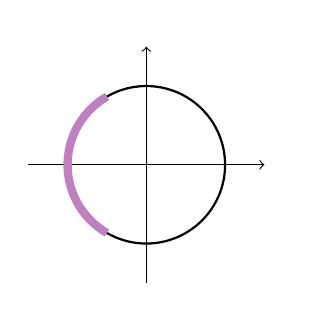
\begin{tikzpicture}
      % Draw the axes
      \draw[->] (-1.5,0) -- (1.5,0) node[right]{};
      \draw[->] (0,-1.5) -- (0,1.5) node[above]{};
    
      % Draw the unit circle
      \draw[thick] (0,0) circle (1);
      
      % Draw the cap of height 1. Its y coordinate is sqrt(1 - 0.5^2) ~ 0.866.
      % \draw[line width=3pt, violet!50] (-0.5, 0.866) arc(90:270:1);
      \draw[line width=3pt, violet!50] (-0.5, 0.866) arc(120:240:1);
    \end{tikzpicture}
    \caption{The unit circle in $\mathbb{R}^2$ with a spherical cap (thick purple arc) of height 0.5. In $\mathbb{R}^d$, the sphere and spherical cap are both $(d-1)$-dimensional objects.}
    \label{fig:cap}
\end{figure}

\begin{lemma}
\label{lem:loss_cap}
    Define height \arxiv{$h(r) = \min\left(r(1-\eps\sigma) + \frac{1 - (\eps\sigma)^2}{2}, 2r\right)$.}
    \narxiv{\begin{equation*}
        h(r) = \min\left(r(1-\eps\sigma) + \frac{1 - (\eps\sigma)^2}{2}, 2r\right).
    \end{equation*}}
    Then $\hat S_{r, 0, h(r)} = V \cap S_{r, 0}$.
\end{lemma}
\begin{proof}
    Orient the 2-dim plane $\text{span}(e_1,e_2)$ so that the positive $e_1$ direction is right and the positive $e_2$ direction is up. Consider the points 0, $e_1$, and some $y \in S_{r,0} \cap H$ where $H$ is the upper half of the $\text{span}(e_1,e_2)$ plane (i.e., $y_2 \geq 0$).  Let $\theta$ be the clockwise angle from $y$ to $e_1$. Proofs of the following claim (and others omitted in this subsection) appear in \Cref{subsec:appendix_upper}.
    \begin{restatable}{claim}{normDiffMonotonicity}
    \label{lem:normDiffMonotonicity}
    $\|y-e_1\|_2 - \|y\|_2$ decreases as $\theta$ decreases.
    \end{restatable}
    
    We want to identify a function $h(r)$ for all $r > 0$ such that $\hat S_{r, 0, h(r)} = V \cap S_{r, 0}$. \Cref{assm:d_sigma} means $\sigma < \frac{1}{\eps}$, so by \Cref{lem:large_sigma}, $V \cap S_{r,0}$ is nonempty. The analysis splits into cases.
    
    \underline{Case 1}: $S_{r,0} \not\subset V$. Since $\frac{1}{\sigma}(\|p - e_1\|_2 - \|p\|_2)$ changes monotonically by \cref{lem:normDiffMonotonicity} then there exists $p = (p_1, p_2, 0,...,0) \in S_{r,0}$ at the base of $\hat S_{r, 0, h(r)}$ such that $\frac{1}{\sigma}(\|p - e_1\|_2 - \|p\|_2) = \eps$. Then $h(r)$ satisfies $(r-h(r))^2 + p_2^2 = r^2$, and we get $p_2 = \sqrt{2h(r)r - h(r)^2}$. 
    
    We can now derive the desired expression for $h(r)$ 
    \begin{restatable}{claim}{expressionOfh}
    \label{lem:expressionOfh}
    $\frac{1}{\sigma}(\|p - e_1\|_2 - \|p\|_2) = \eps$ is equivalent to $h(r) = r(1-\eps \sigma)  + \frac{1 - \eps^2\sigma^2}{2}$
    \end{restatable}
    
    Moreover, we show that with the above definition of $h(r)$, the constraint $h(r) \in [0,2r]$ is equivalent to a constraint on the radius given by $r \geq \frac{1-\eps\sigma}{2}$
    \begin{restatable}{claim}{radiusRangeForValidh}
    \label{lem:radiusRangeForValidh}
    $r(1-\eps \sigma)  + \frac{1 - \eps^2\sigma^2}{2} \in [0, 2r]$ if and only if $r \geq \frac{1-\eps\sigma}{2}$
    \end{restatable}
    
    In summary, $S_{r,0} \not\subset V$ if and only if $r \geq \frac{1-\eps\sigma}{2}$, and for such $r$, we have $\hat S_{r, 0, h(r)} = V \cap S_{r, 0}$ when $h(r)$ is defined as in \cref{lem:expressionOfh}.
    
    \underline{Case 2}: $S_{r,0} \subset V$. By the above, $S_{r,0} \subset V$ if and only if $r < \frac{1-\eps\sigma}{2}$. The statement $S_{r,0} \subset V$ is equivalent to $\frac{1}{\sigma}(\|p - e_1\|_2 - \|p\|_2) = \frac{1}{\sigma}(\sqrt{(r+1)^2 - 2h(r)} - r) \geq \eps$ for all $p \in S_{r,0}$, and this inequality is equivalent to $h(r) \leq r(1-\eps \sigma)  + \frac{1 - \eps^2\sigma^2}{2}$ by replacing equality with inequalities in the proof of \cref{lem:expressionOfh}. By \cref{lem:radiusRangeForValidh}, $r < \frac{1-\eps\sigma}{2}$ is equivalent to $r(1-\eps \sigma) + \frac{1- \eps^2 \sigma^2}{2} > 2r$. Then defining $h(r) = 2r$ suffices to satisfy $h(r) \leq r(1-\eps \sigma)  + \frac{1 - \eps^2\sigma^2}{2}$ for all $r < \frac{1-\eps\sigma}{2}$.
    
    In summary, if we define $h(r)$ as
    \[ h(r) = \begin{cases} 
          r(1-\eps \sigma)  + \frac{1 - \eps^2\sigma^2}{2} & \text{if } r \geq \frac{1-\eps\sigma}{2} \\
          2r & \text{if } r < \frac{1-\eps\sigma}{2} \\
       \end{cases}
    \] 
    then $h(r) \in [0, 2r]$ and $\hat S_{r, 0, h(r)} = V \cap S_{r, 0}$. Since $r(1-\eps \sigma)  + \frac{1 - \eps^2\sigma^2}{2} > 2r$ for $r < \frac{1-\eps\sigma}{2}$, this piecewise function is equivalent to $h(r) = \min\left(r(1-\eps\sigma) + \frac{1 - (\eps\sigma)^2}{2}, 2r\right)$.
\end{proof}

We showed in the above proof that, for small $r$, the entirety of $S_{r,0}$ lies in $V$.
\begin{corollary}
\label{cor:small_r_high_loss}
    If $r \leq \frac{1-\eps \sigma}{2}$, then $S_{r,0} \subset V$.
\end{corollary}

It remains to analyze the high privacy loss region for larger $r$. Our analysis will repeatedly reason about the fraction of a sphere occupied by a cap.

\begin{definition}
\label{def:F}
    Let $F_{r,h}$ denote the fraction of the surface of $S_{r,0}$ occupied by cap $\hat S_{r,0,h}$.
\end{definition}

\begin{lemma}[\cite{L10}]
\label{lem:cap_fraction}
    Let $I_x(a,b) = \frac{\int_0^xt^{a-1}(1-t)^{b-1} dt}{\int_0^1 t^{a-1}(1-t)^{b-1}dt}$ denote the regularized incomplete beta function. Let $h$ be the height function defined in \Cref{lem:loss_cap}. If $h(r) \leq r$, then $F_{r,h(r)} = \frac{1}{2}I_{(2rh(r)-h(r)^2)/r^2}\left(\frac{d-1}{2}, \frac{1}{2}\right)$. If $h(r) > r$, then $F_{r,h(r)} = 1 - F_{r,2r-h(r)}$.
\end{lemma}

There is no closed-form expression for $I_x(a,b)$, but it is a standard function in mathematical libraries like SciPy~\cite{S24}.\footnote{Note that the analytic Gaussian mechanism~\cite{BW18} depends similarly on the standard Gaussian CDF.} We can therefore use \Cref{lem:cap_fraction} to compute the fraction of any $S_{r,0}$ that lies in $V = \cup_{r \in \mathbb{R}^{+}}\hat S_{r,0,h(r)}$ (\Cref{lem:loss_cap}). It remains to extend these results about individual spheres to results about $V$ as a whole.

The next lemma shows that the high-loss cap fraction decreases with $r$. \narxiv{It combines \Cref{lem:loss_cap} and \Cref{lem:cap_fraction} to show directly that the appropriate $I_x(a,b)$ is monotone in $r$ in the desired direction. Since the proof is again mostly calculation, it also appears in \Cref{subsec:appendix_upper}.}

\begin{restatable}{lemma}{FMonotonic}
\label{lem:F_monotonic}
    $F_{r,h(r)}$ is monotone decreasing in $r$.
\end{restatable}
\arxiv{\begin{proof}
    Shorthand $\tau = \eps \sigma$. By \Cref{cor:small_r_high_loss}, $F_{r,h(r)} = 1$ for $r \leq \frac{1-\tau}{2}$. Suppose $r > \frac{1-\tau}{2}$. Then by \Cref{lem:loss_cap}, $h(r) = r(1-\tau) + \frac{1-\tau^2}{2}$.
    
    \underline{Case 1}: $r < \frac{1-\tau^2}{2\tau}$. This rearranges into $-\tau r + \frac{1-\tau^2}{2} > 0$, so $h(r) = r - \tau r + \frac{1-\tau^2}{2} > r$, and $F_{r,h(r)} = 1 - F_{r,2r-h(r)}$. Since we want to prove that $F_{r,h(r)}$ decreases with $r$, it suffices to show that $F_{r,2r-h(r)}$ increases with $r$. By \Cref{lem:cap_fraction},
    \begin{equation*}
        F_{r,2r-h(r)} = \frac{1}{2}I_{(2r[2r-h(r)] - [2r-h(r)]^2)/r^2}\left(\frac{d-1}{2}, \frac{1}{2}\right).
    \end{equation*}
    We expand the subscript for $I$
     \begin{align}
        \frac{2r(2r-h(r)) - (2r-h(r))^2}{r^2} =&\ \frac{4r^2 - 2rh(r) - (4r^2 - 4rh(r) + h(r)^2)}{r^2} \nonumber \\
        =&\ \frac{2rh(r) - h(r)^2}{r^2} \label{eq:h_middle}.
    \end{align}
    Since $h(r) \in [0,2r]$ (\Cref{lem:loss_cap}), $2rh(r) - h(r)^2 \geq 0$. Because $I_x(a, b)$ increases with $x$ for $x \geq 0$, it is enough to show that $[2rh(r) - h(r)^2]/r^2$ increases with $r$. Expanding yields
    \begin{equation*}
        \frac{2rh(r) - h(r)^2}{r^2} = \frac{2r(1-\tau) + (1-\tau^2)}{r} - \frac{r^2(1-\tau)^2 + r(1-\tau)(1-\tau^2) + \frac{(1-\tau^2)^2}{4}}{r^2}.
    \end{equation*}
    We drop terms that don't depend on $r$ to get
    \begin{equation*}
        \frac{1-\tau^2}{r} - \frac{(1-\tau)(1-\tau^2)}{r} - \frac{(1-\tau^2)^2}{4r^2} = (1-\tau^2)\left[\frac{\tau}{r} - \frac{(1-\tau^2)}{4r^2}\right].
    \end{equation*}
    Differentiating the second term with respect to $r$ gives $\frac{1-2\tau r-\tau^2}{2r^3}$. The denominator is always positive, and the numerator  is positive exactly when $r < \frac{1-\tau^2}{2\tau}$.
    
    \underline{Case 2}: $r \geq \frac{1-\tau^2}{2\tau}$. Then $h(r) \leq r$, and
    \begin{equation*}
        F_{r,h(r)} = \frac{1}{2}I_{(2rh(r)-h(r)^2)/r^2}\left(\frac{d-1}{2}, \frac{1}{2}\right).
    \end{equation*}
    By similar logic, it suffices to show that $(2rh(r)-h(r)^2)/r^2$ is decreasing in $r$ for $r \geq \frac{1-\tau^2}{2\tau}$. This follows from the analysis of the previous case.
\end{proof}}

This suggests the following approach: if $M(0)$ samples $y$ with $\|y\|_2 > r$ with probability $p$, then $pF_{r,h(r)}$ is an upper bound on $\P{y\sim M(0)}{y \in V, \|y\|_2 > r}$. The following result gives a closed form for $p$. The expression uses the lower incomplete gamma function and the gamma function, which are also standard functions in mathematical libraries. The proof is mostly calculation and appears in \Cref{subsec:appendix_upper}.

\begin{definition}
\label{def:gammas}
    For $z \geq 0$, the \emph{Gamma function} is $\Gamma(z) = \int_0^\infty t^{z-1}e^{-t} dt$, the \emph{lower incomplete Gamma function} is $\gamma(z, x) = \int_0^x t^{z-1}e^{-t}dt$, and the \emph{upper incomplete Gamma function} is $\Gamma(z, x) = \Gamma(z) - \gamma(z, x)$.
\end{definition} 

\begin{restatable}{lemma}{rBound}
\label{lem:r_bound}
    For $r > 0$, $\P{y \sim M(0)}{\|y\|_2 \leq r} = \frac{\gamma(d, r/\sigma)}{\Gamma(d)}$.
\end{restatable}

The preceding results yield the following upper bound.
\begin{lemma}
\label{lem:upper_bound}
    Suppose \Cref{assm:d_sigma} holds. Let $r_1 < \ldots < r_{n_r}$ where $r_1 =\frac{1-\eps \sigma}{2}$. Then, for $y \sim M(0)$,
    \arxiv{\begin{equation*}
        \P{}{y \in V} \leq \frac{\gamma(d, r_1/\sigma)}{\Gamma(d)} + \sum_{j=1}^{n_r-1}  \frac{\gamma(d, r_{j+1}/\sigma) - \gamma(d, r_j/\sigma)}{\Gamma(d)}F_{r_j, h(r_j)} +  \frac{\Gamma(d, r_{n_r}/\sigma)}{\Gamma(d)}F_{r_{n_r}, h(r_{n_r})}.
    \end{equation*}}
    \narxiv{\begin{align*}
        \P{}{y \in V} \leq&\ \frac{\gamma(d, r_1/\sigma)}{\Gamma(d)} \\
        +&\ \sum_{j=1}^{n_r-1}  \frac{\gamma(d, r_{j+1}/\sigma) - \gamma(d, r_j/\sigma)}{\Gamma(d)}F_{r_j, h(r_j)} \\
        +&\  \frac{\Gamma(d, r_{n_r}/\sigma)}{\Gamma(d)}F_{r_{n_r}, h(r_{n_r})}.
    \end{align*}}
\end{lemma}
\begin{proof}
    The first term is the mass placed on the ball lying entirely in the high privacy loss region (\Cref{cor:small_r_high_loss} and \Cref{lem:r_bound}); the second term is a (left) Riemann sum that upper bounds the mass placed on the high privacy loss region between balls of radius $r_1$ and $r_{n_r}$ (\Cref{lem:cap_fraction}, \Cref{lem:r_bound}, and \Cref{lem:F_monotonic}); and the last is an upper bound on the mass placed on the high privacy loss region outside the ball of radius $r_{n_r}$. More specifically, it is a Riemann sum in which the $j$th approximating rectangle has base length as the $j$th interval on the grid $\left[0, \frac{\gamma(d, r_{1}/\sigma)}{\Gamma(d)},...,\frac{\gamma(d, R_{n_{r}}/\sigma)}{\Gamma(d)},\infty\right]$ and height $F_{r_{j},h(r_{j})}$.
\end{proof}

\Cref{alg:term_1_ub} provides overall upper bound pseudocode.

\begin{algorithm}
    \caption{Term1UpperBound}
    \label{alg:term_1_ub}
    \begin{algorithmic}[1]
    \STATE {\bfseries Input:} Dimension $d$; scale parameter $\sigma$; privacy parameter $\eps$; largest radius $r^*$; number of radii $n_r$
        \IF{$\sigma > 1/\eps$}
            \STATE Return 0 (\Cref{lem:large_sigma})
        \ENDIF
        \IF{$d=1$}
            \STATE Return $1 - \frac{1}{2}\exp\left(\frac{1}{2}\left[\eps - \frac{1}{\sigma}\right]\right)$ (\Cref{lem:one_dim})
        \ENDIF
        \STATE Define $r_1 \gets \frac{1-\eps \sigma}{2}$, $r_{n_r} \gets r^*$, and $r_2, \ldots, r_{n_r-1}$ regularly spaced between $r_1$ and $r_{n_r}$
        \STATE Return upper bound from \Cref{lem:upper_bound}
    \end{algorithmic}
\end{algorithm}

\subsubsection{Second Term Lower Bound}
\label{subsubsec:lb}
\arxiv{It remains to lower bound
\begin{align*}
    \P{y \sim M(1)}{\ell_{M,X',X}(y) \leq -\eps} =&\ \P{y \sim M(1)}{\ln\left(\frac{f_X'(y)}{f_{X}(y)}\right) \leq -\eps} \\
    =&\ \P{y \sim M(1)}{\ln\left(\frac{\exp[-\|y-e_1\|_2 / \sigma]}{\exp[-\|y\|_2 / \sigma]}\right) \leq -\eps} \\
    =&\ \P{y \sim M(1)}{\frac{1}{\sigma}\left(\|y\|_2 - \|y-e_1\|_2\right) \leq -\eps} \\
    =&\ \P{y \sim M(1)}{\frac{1}{\sigma}\left(\|y-e_1\|_2 - \|y\|_2\right) \geq \eps}.
\end{align*}}
\narxiv{It remains to lower bound $\P{y \sim M(1)}{\ell_{M,X',X}(y) \leq -\eps}$. By the same logic used to derive \Cref{eq:plrv_1_ub}, we rewrite it as
\begin{align*}
    &\P{y \sim M(1)}{\ln\left(\frac{f_X'(y)}{f_{X}(y)}\right) \leq -\eps} \\
    =&\ \P{y \sim M(1)}{\frac{1}{\sigma}\left(\|y-e_1\|_2 - \|y\|_2\right) \geq \eps}.
\end{align*}}
The level sets of $M(1)$ are spheres centered at $e_1$. As in the upper bound analysis, there are a few simple cases. The first follows from the same reasoning used for \Cref{lem:large_sigma}.
\begin{corollary}
\label{cor:large_sigma_lb}
    If $\sigma \geq \frac{1}{\eps}$, then $\P{y \sim M(1)}{y \in V} = 0$.
\end{corollary}
The second case uses the same argument as \Cref{lem:one_dim}.
\begin{lemma}
\label{lem:one_dim_lb}
    If $\sigma \leq \frac{1}{\eps}$ and $d = 1$, then $\P{y \sim M(1)}{y \in V} = \frac{1}{2}\exp\left(\frac{1}{2}\left[-\eps - \frac{1}{\sigma}\right]\right)$.
\end{lemma}
\begin{proof}
    $M(1)$ has the same noise density as the Laplace mechanism $\lap{1,\sigma}$, and $|y-e_1| - |y| \geq \sigma \eps$ if and only if $y \leq \frac{1}{2}(1 - \sigma \eps)$. For $z < 1$, the $\lap{1, \sigma}$ CDF is $F(z) = \frac{1}{2}\exp\left(\frac{z-1}{\sigma}\right)$, so by $1 - \sigma \eps \geq 0$, $\P{y \sim M(1)}{y \in V} = \frac{1}{2}\exp\left(\frac{1}{2}\left[-\eps - \frac{1}{\sigma}\right]\right)$.
\end{proof}
We therefore work under \Cref{assm:d_sigma} for the rest of this section. The remaining analysis reasons about specific spheres $S_{R,1}$.
\begin{definition}
\label{def:U_R}
    For $R > 0$, define $U_R$ to be the fraction of $S_{R,1}$ contained in $V$.
\end{definition}
We start by identifying when $U_R = 0$.
\begin{lemma}
\label{lem:U_R_0}
    If $0 < R < \frac{1+\eps \sigma}{2}$, then $U_{R} = 0$. 
\end{lemma}
\begin{proof}
    Shorthand $\tau = \eps \sigma$ for neatness. By \Cref{cor:small_r_high_loss}, $F_{r,h(r)} = 1$ for $r \leq \frac{1-\tau}{2}$. Let $r_1 = \frac{1-\tau}{2}$ denote the largest radius such that $F_{r,h(r)} = 1$. This shows that the point with the largest $e_1$-coordinate in $V \cap S_{r,0}$ has $e_1$-coordinate $r$ for $0 < r \leq r_1$. For $r > r_1$, the point with the largest $e_1$-coordinate in $V \cap S_{r,0}$ has $e_1$-coordinate $-r + h(r) = -r\tau + \frac{1-\tau^2}{2}$ which is monotonically decreasing as $r$ increases. Overall, the point with the largest $e_1$-coordinate in $V \cap S_{r,0}$ is increasing for $0 < r \leq r_1$ and decreasing for $r > r_1$, so $r_1$ is the maximum $e_1$-coordinate of this point over all radii.
    
    It follows that $0 < R < 1 - r_{1}$ implies $S_{R,1} \cap S_{r,0} = \emptyset$ for all $r > 0$, and since $V \subset \cup_{r \in \mathbb{R}^{+}}S_{r,0}$, we get $U_{R} = 0$.
\end{proof}

It remains to handle the large $R$ case. We will show that, as was the case in the upper bound analysis, each $S_{R,1} \cap V$ is a spherical cap on $S_{R,1}$. The first result proves that $S_{R,1} \cap V$ has this form. This result is not technically necessary for the rest of the argument, but it explains why we attempt to solve for $S_{R,1} \cap V$ as a cap later.

\begin{lemma}
\label{lem:lower_bound_cap_exists}
    For $R \geq \frac{1+\eps \sigma}{2}$, $S_{R,1} \cap V$ is a spherical cap $\hat S_{R,1,H(R)}$.
\end{lemma}
\begin{proof}
    Shorthand $\tau = \eps \sigma$. Recall from \cref{lem:large_sigma} that $V$ is the convex hull of the $-e_1$ facing component of a hyperboloid with foci $0$ and $e_1$ and with constant difference $\tau$. To see why $S_{R,1} \cap V$ is a spherical cap, observe that both the hyperboloid-bounded region $V$ and $S_{R,1}$ are symmetric around $e_1$, so their intersection must be symmetric around $e_1$ as well. Let $P_{v_1, v_2}$ denote projection onto $\text{span}(v_1, v_2)$. Then $P_{e_1,e_2}(V) \cap P_{e_1,e_2}(S_{R,1})$ is a 1-dimensional spherical cap of some height $H$ in $P_{e_1,e_2}(S_{R,1})$. Since $V \cap S_{R,1}$ is symmetric around $e_1$, the previous sentence also holds if we replace $P_{e_1,e_2}$ with $P_{e_1, v}$ for any $v$ orthogonal to $e_1$. Thus $V \cap S_{R,1} = \cup_{v \perp e_1}P_{e_1,v}(V) \cap P_{e_1,v}(S_{R,1}) = \hat{S}_{R,1,H}$.
\end{proof}

It remains to identify the $H$ referenced in \Cref{lem:lower_bound_cap_exists}.\narxiv{ To do so, we start with an arbitrary $y \in S_{R,1}$ and solve for an $e_1$ coordinate $X$ such that $y_1 \leq X$ if and only if $y_1 \leq -\|y\|_2 + h(\|y\|_2)$ (\Cref{lem:loss_cap}). The bulk of the proof beyond this idea is algebraic manipulation, so it appears in \Cref{subsec:appendix_lower}.}
\begin{restatable}{lemma}{lowerCap}
\label{lem:e1_cap}
    Define $X = \frac{1+(\eps \sigma)^2-2\eps \sigma R}{2}$ and $H(R) = R-1+X$. Then cap $\hat S_{R, 1, H(R)} = S_{R,1} \cap V$.
\end{restatable}
\arxiv{\begin{proof}
    To verify this, we start with an arbitrary $y \in S_{R,1}$ and attempt to determine a cutoff $X \in \mathbb{R}$ such that $y \in V$ iff $y_1 \leq X$. For any two points $y,y' \in S_{R,1}$ such that $y_1 = y_{1}'$, it is true that $y \in V$ iff $y' \in V$ since $V$ is spherically symmetric around $e_1$. If $y' = y_{1}e_{1} + v$ for some $v$ orthogonal to $e_1$, then by $S_{R,1}$'s spherical symmetry around $e_1$, the point $y = y_{1}e_{1} + |v|e_2$ is also in $S_{R,1}$. Therefore, our goal is to find the minimum cutoff $X$ for the point $y = (y_1, y_2, 0,...,0)$ such that $y \in V$ iff $y_{1} \leq X$.
    
    We know $y \in S_{r',0}$ for some $r' > 0$. Since $y_1^2 + y_2^2 = r'^2$, and $y \in S_{R,1}$ implies $(y_1-1)^2 + y_2^2 = R^2$, then combining these yields $r' = \sqrt{R^2+2y_1-1}$. Thus we have $y \in V$ if and only if $y_1 \leq -r' + h(r')$. By \Cref{lem:loss_cap}, $-r' + h(r') = \min(-\tau r' + \frac{1-\tau^2}{2}, 2r')$. We have $-\tau r' + \frac{1-\tau^2}{2} = -\tau\sqrt{R^2+2y_1-1} + \frac{1-\tau^2}{2}$,
    so we solve for the largest $X$ where $X \leq  \min(-\tau\sqrt{R^2+2X-1} + \frac{1-\tau^2}{2}, 2\sqrt{R^2+2X-1})$.
    
    Solving for $X$ under the first constraint yields 
    \begin{align}
        \left(X - \frac{1-\tau^2}{2}\right)^2 \geq&\ \tau^2(R^2+2X-1) \nonumber \\
        X^2 - X(1+\tau^2) + \frac{\tau^4-2\tau^2+1 - 4\tau^2R^2 + 4\tau^2}{4} \geq&\ 0 \nonumber \\
        X^2 - X(1+\tau^2) + \frac{\tau^4+2\tau^2+1 - 4\tau^2R^2}{4} \geq&\ 0 \label{eq:X_inequality}.
    \end{align}
    The roots of the LHS are given by 
    \begin{equation*}
        X =\frac{1 + \tau^2 \pm \sqrt{(1+\tau^2)^2 - ([1+\tau^2]^2 - 4\tau^2R^2)}}{2} \\
        =\frac{1 + \tau^2 \pm 2\tau R}{2}.
    \end{equation*}
    Let $x_1 = \frac{1+\tau^2 -2\tau R}{2}$ and $x_2 = \frac{1+\tau^2 + 2\tau R}{2}$. As the LHS of \Cref{eq:X_inequality} is a convex parabola, the inequality is satisfied on the intervals $(-\infty, x_1] \cup [x_2, \infty)$. But the first constraint on $X$ also implies the weaker inequality $X < \frac{1-\tau^2}{2}$ so $X \notin [x_2, \infty)$. Then $x_1$ is the largest value that satisfies the first constraint.
    
    For any $X \in (x_1, x_2)$, we have $X > -\tau\sqrt{R^2+2X-1} + \frac{1-\tau^2}{2} \geq \min(-\tau\sqrt{R^2+2X-1} + \frac{1-\tau^2}{2}, 2\sqrt{R^2+2X-1})$. So if we can show that $x_1 \leq 2\sqrt{R^2+2x_{1}-1}$, then $x_1$ will indeed be the desired cutoff. We actually prove a stronger inequality
    \begin{align*}
        x_1 \leq&\ \sqrt{R^2+2x_{1}-1} \\
        \frac{1+\tau^2 - 2\tau R}{2} \leq&\ R - \tau \\
        (1+\tau)^2 \leq&\ 2R(1 + \tau) \\
        \frac{1+\tau}{2} \leq&\ R
    \end{align*}
    which follows from our starting assumption on $R$. So $X = \frac{1+\tau^2 -2\tau R}{2}$ is the desired cutoff. This leads to a cap on $S_{R,1}$ of height
    \begin{equation*}
        H(R) = X-(1-R) = \frac{1+\tau^2 -2\tau R}{2} - 1 + R = R(1-\tau) - \frac{1-\tau^2}{2}.
    \end{equation*}
    The last step is verifying that this is a valid height lying in $[0,2R]$. The lower bound follows from $R(1-\tau) \geq \frac{1-\tau^2}{2}$ rearranging into the starting assumption $R \geq \frac{1+\tau}{2}$. We prove a stronger upper bound of $R$ by rearranging
    \begin{align*}
        R(1-\tau) - \frac{1-\tau^2}{2} \leq&\ R \\
        -\frac{1-\tau^2}{2} \leq& \tau R
    \end{align*}
    which uses $0 < \tau <1$ and $R > 0$.
\end{proof}}

\begin{lemma}
\label{lem:U_R_monotonic}
    If $R \geq \frac{1+\eps \sigma}{2}$, then $U_R$ is monotone increasing in $R$.
\end{lemma}
\begin{proof}
    Shorthand $\tau = \eps \sigma$. \Cref{lem:U_R_0} established that $U_R = 0$ for $R < \frac{1+\tau}{2}$, so it remains to show that $U_R$ is increasing in $R$ for $R \geq \frac{1+\tau}{2}$. The proof of \Cref{lem:e1_cap} established that $H(R) \in [0,R]$, so we apply \Cref{lem:cap_fraction} to get that $\hat S_{R, 1, H(R)}$ occupies a fraction of $S_{R,1}$ given by $\frac{1}{2}I_{(2RH(R) - H(R)^2)/R^2}\left(\frac{d-1}{2}, \frac{1}{2}\right)$. By the same logic used in the proof of \Cref{lem:F_monotonic}, we can show that $U_{R}$ is monotone increasing by verifying that the expression in the $I$ subscript is nonnegative and increasing in $R$.
    
    The first condition follows from the aforementioned result $H(R) \leq R$. For the second condition,
    \arxiv{\begin{align*}
        \frac{2R[R-1+X] - [R-1+X]^2}{R^2} =&\ \frac{2R^2 - 2R + 2XR - [R^2 - 2R + 2XR + 1 -2X + X^2]}{R^2} \\
        =&\ \frac{R^2 - 1 + 2X - X^2}{R^2} \\
        =&\ 1 - \left(\frac{X-1}{R}\right)^2 \\
        =&\ 1 - \left(\frac{\tau^2 - 2\tau R - 1}{2R}\right)^2.
    \end{align*}}
    \narxiv{\begin{align*}
        &\frac{2R[R-1+X] - [R-1+X]^2}{R^2} \\
        =&\ \frac{R^2 - 1 + 2X - X^2}{R^2} \\
        =&\ 1 - \left(\frac{X-1}{R}\right)^2 \\
        =&\ 1 - \left(\frac{\tau^2 - 2\tau R - 1}{2R}\right)^2.
    \end{align*}}
    We wanted to prove that this expression is increasing in $R$, so we show that the second term is decreasing in $R$. Taking its derivative with respect to $R$ yields
    \arxiv{\begin{equation*}
        2\left(\frac{\tau^2 - 2\tau R - 1}{2R}\right) \cdot \frac{2R(-2\tau) - 2(\tau^2 - 2\tau R - 1)}{4R^2} = \left(\frac{\tau^2 - 2\tau R - 1}{R}\right) \cdot \frac{1-\tau^2}{2R^2}.
    \end{equation*}}
    \narxiv{\begin{align*}
        &2\left(\frac{\tau^2 - 2\tau R - 1}{2R}\right) \cdot \frac{2R(-2\tau) - 2(\tau^2 - 2\tau R - 1)}{4R^2} \\
        =&\ \left(\frac{\tau^2 - 2\tau R - 1}{R}\right) \cdot \frac{1-\tau^2}{2R^2}.
    \end{align*}}
    Because $R > 0$ and $0 < \tau < 1$, the numerator of the first term is negative, and the remaining terms are positive, so the entire quantity is negative.
\end{proof}

Since we want to lower bound the mass on these $U_R$, we use \Cref{lem:r_bound} and employ a left Riemann sum in which the $j$th approximating rectangle has base length as the $j$th interval on the grid $\left[\frac{\gamma(d, R_{1}/\sigma)}{\Gamma(d)},...,\frac{\gamma(d, R_{n_{R}}/\sigma)}{\Gamma(d)},\infty\right]$ and has height $F_{R_{j},H(R_{j})}$. The proof of the following result uses similar logic as the proof of \Cref{lem:upper_bound}.

\begin{lemma}
\label{lem:lower_bound}
    Suppose \Cref{assm:d_sigma} holds. Let $R_1 < \ldots < R_{n_R}$ where $R_1 = \frac{1+\tau}{2}$. Then for $y \sim M(1)$,
    \arxiv{\begin{equation*}
        \P{}{y \in V} \geq \sum_{j=1}^{n_R-1} \frac{\gamma(d, R_{j+1}/\sigma) - \gamma(d,R_j/\sigma)}{\Gamma(d)}F_{R_j, H(R_j)} + \frac{\Gamma(d, R_{n_{R}}/\sigma)}{\Gamma(d)}F_{R_{n_{R}},H(R_{n_R})}
    \end{equation*}}
    \narxiv{\begin{align*}
        \P{}{y \in V} \geq&\ \sum_{j=1}^{n_R-1} \frac{\gamma(d, R_{j+1}/\sigma) - \gamma(d,R_j/\sigma)}{\Gamma(d)}F_{R_j, H(R_j)} \\
        &+ \frac{\Gamma(d, R_{n_{R}}/\sigma)}{\Gamma(d)}F_{R_{n_{R}},H(R_{n_R})}
    \end{align*}}
    where we reused the definition of $F$ from \Cref{def:F}.
\end{lemma}

\Cref{alg:term_2_lb} provides overall lower bound pseudocode.

\begin{algorithm}
    \caption{Term2LowerBound}
    \label{alg:term_2_lb}
    \begin{algorithmic}[1]
    \STATE {\bfseries Input:} Dimension $d$; scale parameter $\sigma$; privacy parameter $\eps$; largest radius $R^*$; number of radii $n_R$
    \IF{$\sigma \geq 1/\eps$}
        \STATE Return 0 (\Cref{cor:large_sigma_lb})
    \ENDIF
    \IF{$d=1$}
        \STATE Return $\frac{1}{2}\exp\left(\frac{1}{2}\left[-\eps - \frac{1}{\sigma}\right]\right)$ (\Cref{lem:one_dim_lb})
    \ENDIF
    \STATE Define $R_1 \gets \frac{1+\tau}{2}$, $R_{n_R} \gets R^*$, and $R_2, \ldots, R_{n_R-1}$ regularly spaced between $R_1$ and $R_{n_R}$
    \STATE Return lower bound from \Cref{lem:lower_bound}
    \end{algorithmic}
\end{algorithm}

\subsubsection{Overall Algorithm}
\label{subsec:overall}
\Cref{alg:term_1_ub} upper bounds the first term in the inequality in \Cref{lem:approx_dp} and \Cref{alg:term_2_lb} lower bounds the second term. This upper bounds the LHS of the inequality, so if it is at most $\delta$, then the mechanism is $(\eps, \delta)$-DP.

The last step is choosing $n_r$, $r^*$, $n_R$, and $R^*$. Our experiments suggests that setting $n_r = n_R = 1000$ yields a reasonably tight approximation for $d \leq 100$ (see \Cref{subsec:experiments_privacy}); larger values should only be tighter, at the cost of speed. We choose $r^*$ using \Cref{lem:r_bound} so $\P{y \sim M(0)}{\|y\|_2 > r^*} = \frac{\delta}{100}$; in the context of \Cref{lem:upper_bound}, we use $F_{r_{n_r}, h(r_{n_r})}$ to upper bound the cap fraction for all $S_{r,0}$ with $r \geq r_{n_r}$, so we choose $r^*$ to make the effect of this approximation negligible. By the same logic, we use $R^* = r^*$.

\Cref{alg:overall} collects the entire process into pseudocode.

\begin{algorithm}
    \caption{CheckApproximateDP}
    \label{alg:overall}
    \begin{algorithmic}[1]
    \STATE {\bfseries Input:} Dimension $d$; scale parameter $\sigma$; privacy parameters $\eps$, $\delta$; numbers of radii $n_r$, $n_R$
    \STATE Compute $r^*$ such that $\P{y \sim M(0)}{\|y\|_2 > r^*} = \frac{\delta}{100}$ (\Cref{lem:r_bound})
    \STATE $T_1 \gets \text{Term1UpperBound}(d, \sigma, \eps, r^*, n_r)$
    \STATE $T_2 \gets \text{Term2LowerBound}(d, \sigma, \eps, r^*, n_R)$
    \STATE Return $(T_1 - e^\eps T_2 \leq \delta)$
    \end{algorithmic}
\end{algorithm}